\documentclass[11pt]{article}

\usepackage{kotex}
\usepackage{graphicx}
\usepackage{gensymb}

\begin{document}
Hello World!

\begin{figure}[b]
\centering\includegraphics[scale=0.5]{../images/eps.png}
\caption{\texttt{\symbol{92}includegraphics} 명령으로 부른 그램(축소/확대) \label{fig:eps01}}
\end{figure}

\begin{figure}
\centering\includegraphics[width=.97\textwidth, height=5cm]{../images/eps.png}
\caption{\texttt{\symbol{92}includegraphics} 명령의 그림 크기 조절 \label{fig:eps02}}
\end{figure}

\begin{figure}[t]
\caption{\texttt{\symbol{92}includegraphics}로 그림 일부만 잘라오기 \label{fig:eps03}}
\centering\includegraphics*[300pt, 0pt][600pt, 150pt]{../images/eps.png}
\end{figure}

\begin{figure}[t]
\caption{\texttt{\symbol{92}includegraphics*} 명령의 잘라오기 및 그림 크기 변경 \label{fig:eps04}}
\centering\includegraphics*[bb=300 0 600 150, width=0.5\textwidth, height=0.4\textwidth]{../images/eps.png}
\end{figure}

\begin{figure}[t]
\begin{center}
\includegraphics[width=1.8in]{../images/eps.png}
\includegraphics[width=1.8in, angle=-30]{../images/eps.png}
caption{PostScript 그림 \texttt{eps.png}의 원본 및 반시계 방향으로 30 \degree 회전한 결과 \label{fig:sunrise}}
\end{center}
\end{figure}

\begin{figure}[t]
왼쪽 문자--
\includegraphics*[bb=0 0 150 305]{../images/eps.png}
--오른쪽 문자
\caption{\texttt{*} 있는 \texttt{\symbol{92}includegraphics*} 명령 \label{fig:include*}}
\end{figure}

\begin{figure}[t]
외쪽 문자--
\includegraphics[bb=0 0 150 300]{../images/eps.png}
--오른쪽 문자
\caption{\texttt{*} 없는 \texttt{\symbol{92}includegraphics} 명령 \label{fig:include0}}
\end{figure}

\includegraphics[width=0.5\textwidth, page=5]{../images/style.pdf}



\end{document}